\documentclass[12pt,a4paper]{article}
% Packages
\usepackage[utf8]{inputenc}
\usepackage[T1]{fontenc}
\usepackage{amsmath}
\usepackage{amssymb}
\usepackage{graphicx}
\usepackage{booktabs}
\usepackage{array}
\usepackage{hyperref}
\usepackage{listings}
\usepackage{xcolor}
\usepackage{tikz}
\usepackage{caption}
\usepackage{subcaption}
\usepackage{multirow}
\usepackage{tabularx}
\usepackage{float}
\usepackage[margin=2cm]{geometry}
\usepackage{helvet}
\renewcommand{\familydefault}{\sfdefault}
\usepackage{titlesec}
\usetikzlibrary{positioning,shapes.geometric,arrows.meta}

% IEEE-style section formatting (left-aligned)
\titleformat{\section}{\normalfont\Large\bfseries}{\thesection}{1em}{}
\titleformat{\subsection}{\normalfont\large\bfseries}{\thesubsection}{1em}{}
\titleformat{\subsubsection}{\normalfont\normalsize\bfseries}{\thesubsubsection}{1em}{}



% Dark theme code listing styles
\definecolor{codebg}{RGB}{40,42,54}
\definecolor{codecomment}{RGB}{98,114,164}
\definecolor{codestring}{RGB}{241,250,140}
\definecolor{codekeyword}{RGB}{255,121,198}
\definecolor{codenumber}{RGB}{189,147,249}
\definecolor{codetext}{RGB}{248,248,242}
\definecolor{codegreen}{RGB}{80,250,123}

\lstdefinestyle{codestyle}{
    basicstyle=\ttfamily\footnotesize\color{codetext},
    keywordstyle=\color{codekeyword}\bfseries,
    commentstyle=\color{codecomment}\itshape,
    stringstyle=\color{codestring},
    numberstyle=\tiny\color{codenumber},
    breaklines=true,
    frame=single,
    backgroundcolor=\color{codebg},
    rulecolor=\color{codebg},
    numbers=left,
    numbersep=8pt,
    xleftmargin=15pt,
    framexleftmargin=15pt,
    showstringspaces=false
}

\lstdefinestyle{bashstyle}{
    language=bash,
    basicstyle=\ttfamily\footnotesize\color{codetext},
    keywordstyle=\color{codekeyword},
    commentstyle=\color{codecomment},
    stringstyle=\color{codestring},
    breaklines=true,
    frame=single,
    backgroundcolor=\color{codebg},
    rulecolor=\color{codebg},
    showstringspaces=false
}

\lstdefinestyle{pythonstyle}{
    language=Python,
    basicstyle=\ttfamily\footnotesize\color{codetext},
    keywordstyle=\color{codekeyword}\bfseries,
    commentstyle=\color{codecomment}\itshape,
    stringstyle=\color{codestring},
    breaklines=true,
    frame=single,
    backgroundcolor=\color{codebg},
    rulecolor=\color{codebg},
    showstringspaces=false,
    morekeywords={self,True,False,None}
}

\lstdefinestyle{cppstyle}{
    language=C++,
    basicstyle=\ttfamily\footnotesize\color{codetext},
    keywordstyle=\color{codekeyword}\bfseries,
    commentstyle=\color{codecomment}\itshape,
    stringstyle=\color{codegreen},
    breaklines=true,
    frame=single,
    backgroundcolor=\color{codebg},
    rulecolor=\color{codebg},
    numbers=left,
    numberstyle=\tiny\color{codenumber},
    numbersep=8pt,
    xleftmargin=15pt,
    framexleftmargin=15pt,
    showstringspaces=false,
    morekeywords={int,void,class,public,private,return,if,for,while,break}
}

% Hyperref setup
\hypersetup{
    colorlinks=true,
    linkcolor=blue,
    citecolor=blue,
    urlcolor=blue
}

% Header and footer setup
\usepackage{fancyhdr}
\setlength{\headheight}{14.5pt}
\addtolength{\topmargin}{-2.5pt}
\pagestyle{fancy}
\fancyhf{}
\fancyhead[L]{William Park}
\fancyhead[R]{Survey on Parallel Subgraph Matching}
\fancyfoot[R]{\thepage}
\renewcommand{\headrulewidth}{0.4pt}
\renewcommand{\footrulewidth}{0pt}

% Also apply to chapter pages
\fancypagestyle{plain}{
    \fancyhf{}
    \fancyhead[L]{William Park}
    \fancyhead[R]{Survey on Parallel Subgraph Matching}
    \fancyfoot[R]{\thepage}
    \renewcommand{\headrulewidth}{0.4pt}
}

% Start page numbering at 37 and chapter at 5
\setcounter{page}{42}
\setcounter{section}{4}

\begin{document}

%==============================================================================
\section{Benchmarking Framework Architecture}
\label{ch:framework}
%==============================================================================

A critical challenge in comparative evaluation of parallel subgraph isomorphism algorithms is the heterogeneity of implementations: each algorithm employs different input formats, command-line interfaces, output conventions, and configuration mechanisms. To enable fair and consistent comparison, we developed a unified benchmarking framework based on the \emph{Controller-Adapter} design pattern.

\subsection{Design Pattern: Controller-Adapter Architecture}

The Controller-Adapter pattern provides a clean abstraction layer between the benchmarking logic and algorithm-specific implementation details. This architecture comprises three principal components:

\begin{enumerate}
    \item \textbf{Master Controller}: A central orchestration module that coordinates experiment execution, manages configuration, and aggregates results.
    \item \textbf{Unified Interface}: An abstract specification defining the contract that all algorithm adapters must implement.
    \item \textbf{Algorithm Adapters}: Concrete implementations that wrap each algorithm's binary executable and translate between the unified interface and algorithm-specific conventions.
\end{enumerate}

Figure~\ref{fig:adapter-architecture} illustrates the architectural hierarchy.

\begin{figure}[htbp]
\centering
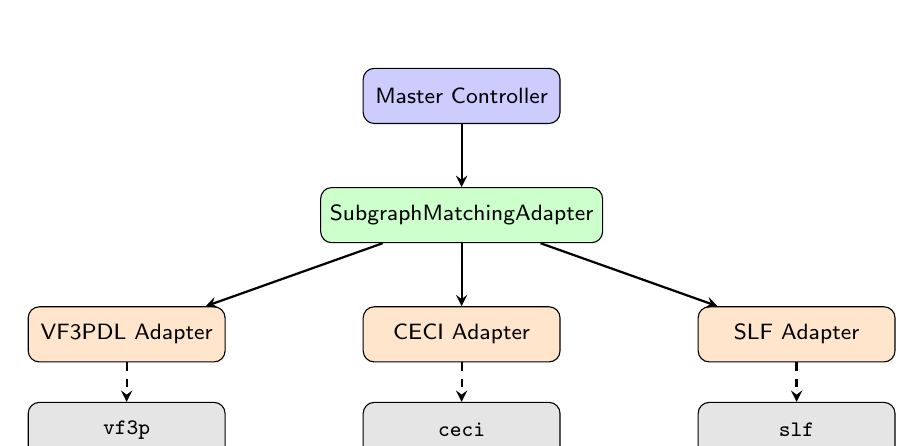
\begin{tikzpicture}[
    node distance=0.8cm,
    box/.style={rectangle, draw, rounded corners, minimum width=2.5cm, minimum height=0.7cm, align=center, font=\footnotesize},
    arrow/.style={->, >=stealth, thick}
]
% Controller
\node[box, fill=blue!20] (ctrl) {Master Controller};
% Interface
\node[box, fill=green!20, below=of ctrl] (iface) {SubgraphMatchingAdapter};
% Adapters
\node[box, fill=orange!20, below left=0.8cm and 1.2cm of iface] (vf3) {VF3PDL Adapter};
\node[box, fill=orange!20, below=of iface] (ceci) {CECI Adapter};
\node[box, fill=orange!20, below right=0.8cm and 1.2cm of iface] (slf) {SLF Adapter};
% Binaries
\node[box, fill=gray!20, below=0.5cm of vf3] (vf3bin) {\texttt{vf3p}};
\node[box, fill=gray!20, below=0.5cm of ceci] (cecibin) {\texttt{ceci}};
\node[box, fill=gray!20, below=0.5cm of slf] (slfbin) {\texttt{slf}};
% Arrows
\draw[arrow] (ctrl) -- (iface);
\draw[arrow] (iface) -- (vf3);
\draw[arrow] (iface) -- (ceci);
\draw[arrow] (iface) -- (slf);
\draw[arrow, dashed] (vf3) -- (vf3bin);
\draw[arrow, dashed] (ceci) -- (cecibin);
\draw[arrow, dashed] (slf) -- (slfbin);
\end{tikzpicture}
\caption{Controller-Adapter architecture. Solid arrows: method calls; dashed arrows: subprocess execution.}
\label{fig:adapter-architecture}
\end{figure}

\subsection{Standardising Input Format}

Table~\ref{tab:formats} summarises the input format requirements for each algorithm.

\begin{table}[htbp]
\centering
\caption{Input format specifications for evaluated algorithms.}
\label{tab:formats}
\begin{tabular}{llll}
\toprule
\textbf{Algorithm} & \textbf{Format} & \textbf{Type} & \textbf{Structure} \\
\midrule
VF3P & VF3/Adjacency & Text & Adjacency list \\
CECI & HKU/Edge List & Text & Edge list with header \\
SLF & VF3/Adjacency & Text & Adjacency list \\
\bottomrule
\end{tabular}
\end{table}

\paragraph{VF3/Adjacency Format.}
The VF3 format represents graphs as adjacency lists. The first line specifies the vertex count, followed by vertex definitions (ID and label), then for each vertex, the edge count and incident edges:

\begin{lstlisting}[style=bashstyle]
8                    # Number of vertices
0 1                  # Vertex 0, label 1
1 1                  # Vertex 1, label 1
5                    # Vertex 0 has 5 edges
0 1                  # Edge 0 -> 1
0 2                  # Edge 0 -> 2
\end{lstlisting}

\paragraph{HKU/Edge List Format.}
The HKU format employs an explicit edge list representation:

\begin{lstlisting}[style=bashstyle]
t # 0                # Graph identifier
v 0 1                # Vertex 0, label 1
v 1 1                # Vertex 1, label 1
e 0 1 0              # Edge from 0 to 1, label 0
e 0 2 0              # Edge from 0 to 2, label 0
\end{lstlisting}

\subsection{Adapter Implementation}

Each adapter implements the \texttt{SubgraphMatchingAdapter} abstract base class:

\begin{lstlisting}[style=pythonstyle]
class SubgraphMatchingAdapter(ABC):
    @abstractmethod
    def run(self, query_path: str, data_path: str,
            threads: int, timeout: int,
            solution_limit: int) -> BenchmarkResult:
        """Execute subgraph matching."""
        pass

    @abstractmethod
    def get_graph_format(self) -> str:
        """Return expected input format identifier."""
        pass
\end{lstlisting}

\subsection{Master Controller Operation}

The master controller implements experiment orchestration through nested iteration over the experimental parameter space:

\begin{lstlisting}[style=pythonstyle]
for algorithm in algorithms:
    adapter = get_adapter(algorithm)
    for dataset in datasets:
        for query in queries[dataset]:
            for threads in thread_counts:
                result = adapter.run(
                    query, data_graph[dataset],
                    threads, TIMEOUT, LIMIT)
                append_to_csv(result)
\end{lstlisting}

\subsection{Standardised Output Format}

All adapters produce results conforming to a unified CSV schema:

\begin{lstlisting}[style=bashstyle]
Algorithm,Dataset,Query,Threads,Time_s,Solutions,Memory_MB,Status
VF3-O,enron,query_dense_8v_1,8,0.234,15420,128.5,SUCCESS
CECI,enron,query_dense_8v_1,8,0.187,15420,145.2,SUCCESS
SLF,enron,query_dense_8v_1,8,0.156,15420,112.8,SUCCESS
\end{lstlisting}

%==============================================================================
\section{Experimental Setup}
\label{ch:setup}
%==============================================================================

\subsection{Hardware Environment}

\paragraph{Primary Server.}
All experiments were conducted on TODS1 (\texttt{tods1.cse.unsw.edu.au}), a shared server in the UNSW CSE department with the following specifications:

\begin{itemize}
    \item \textbf{CPUs}: 96 logical cores (48 physical cores with hyperthreading)
    \item \textbf{Architecture}: 2 NUMA nodes (Node 0: cores 0--23, 48--71; Node 1: cores 24--47, 72--95)
    \item \textbf{Memory}: 502 GB shared RAM
\end{itemize}

\paragraph{Development Environment.}
Local testing and development was performed on a MacBook Air M2 (8GB RAM).

\subsection{Software Environment}

\begin{itemize}
    \item \textbf{Language}: C++
    \item \textbf{Parallelisation}: OpenMP
    \item \textbf{Compiler}: GCC (standard Linux toolchain on Ubuntu)
    \item \textbf{Build System}: Make
\end{itemize}

\subsection{Experimental Parameters}

\begin{table}[htbp]
\centering
\caption{Experimental parameters.}
\label{tab:parameters}
\begin{tabular}{ll}
\toprule
\textbf{Parameter} & \textbf{Value} \\
\midrule
Thread counts & 1, 2, 4, 8, 16, 32, 64 \\
Match limit ($K$) & 50 million (500M for select tests) \\
Timeout & 600 seconds (10 minutes) \\
\bottomrule
\end{tabular}
\end{table}

\subsection{Datasets}

Table~\ref{tab:datasets} describes the graph datasets used in our evaluation.

\begin{table}[htbp]
\centering
\caption{Dataset characteristics.}
\label{tab:datasets}
\begin{tabular}{llrr}
\toprule
\textbf{Dataset} & \textbf{Type} & \textbf{Vertices} & \textbf{Edges} \\
\midrule
ENRON & Email network & $\sim$37K & $\sim$368K \\
DBLP & Collaboration network & $\sim$317K & $\sim$1M \\
LiveJournal & Social network & $\sim$4M & $\sim$35M \\
RoadNet-CA & Road network & $\sim$2M & $\sim$5.5M \\
\bottomrule
\end{tabular}
\end{table}

\subsection{Query Patterns}

Query patterns were generated with the following characteristics:

\begin{itemize}
    \item \textbf{Densities}: Sparse, Dense
    \item \textbf{Sizes}: 8, 16, 24, 32 vertices
    \item \textbf{Format}: 5 queries per (density $\times$ size) combination
\end{itemize}

\subsection{Algorithms Compared}

Table~\ref{tab:algorithms} summarises the algorithms evaluated in this study.

\begin{table}[htbp]
\centering
\caption{Evaluated algorithms and their parallelisation strategies.}
\label{tab:algorithms}
\begin{tabular}{lp{4cm}}
\toprule
\textbf{Algorithm} & \textbf{Parallelisation Strategy} \\
\midrule
VF3PDL & Domain decomposition with descendant limit \\
SLF & Passive work sharing with depth priority \\
CECI & Index-based intersection \\
\bottomrule
\end{tabular}
\end{table}

\subsection{Research Questions}

This evaluation addresses three research questions:

\begin{enumerate}
    \item[\textbf{RQ1}:] How do parallel subgraph matching algorithms scale, and what limits their speedup?
    \item[\textbf{RQ2}:] How do graph density and topology affect the relative performance of traversal-based (SLF/VF3) versus index-based (CECI) algorithms?
    \item[\textbf{RQ3}:] Is there a fundamental tradeoff between pruning effectiveness and parallel scalability?
\end{enumerate}

%==============================================================================
\section{Experimental Results}
\label{ch:results}
%==============================================================================

%------------------------------------------------------------------------------
\subsection{Research Question 1: Parallel Scaling Behaviour}
\label{sec:rq1}
%------------------------------------------------------------------------------

This section addresses Research Question 1: How do parallel subgraph matching algorithms scale, and what limits their speedup? The analysis evaluates three algorithms: VF3 (specifically the VF3PDL implementation), CECI, and SLF.

Parallel speedup is formally defined as $S_p = T_1 / T_p$, where $T_1$ is sequential execution time and $T_p$ is parallel execution time on $p$ processors. The theoretical upper bound establishes that $T_1 \leq p \cdot T_p$, implying linear speedup ($S_p = p$) as the maximum achievable under ideal conditions. Superlinear speedup ($S_p > p$) can occur in search problems due to work anomalies, where parallel exploration collectively avoids unproductive regions.

\subsection{Memory Constraints and Scalability Limits}

\begin{figure}[htbp]
\centering
\includegraphics[width=0.9\textwidth]{rq1_memory_scaling.png}
\caption{Memory consumption scaling from 1 to 64 threads across datasets.}
\label{fig:rq1-memory}
\end{figure}

This experiment examines the memory consumption of each algorithm as thread counts increase from 1 to 64. The results indicate a significant divergence in resource management strategies between traversal-based and index-based approaches.

VF3 exhibits a strictly linear increase in memory consumption relative to thread count. On the RoadNet dataset with dense 8-vertex queries, memory usage increases from approximately 1.6 GB at 1 thread to 43 GB at 64 threads, representing a 27-fold increase. The growth is even more pronounced on DBLP, escalating from 272 MB to 10.3 GB (38-fold increase). This demonstrates that VF3 allocates deep copies of state for each worker, creating a hard scalability limit on memory-constrained systems.

CECI, in contrast, maintains a constant memory footprint regardless of thread count. Usage remains stable at approximately 125 MB for RoadNet and 63 MB for DBLP across all thread counts. This indicates that CECI threads operate on a shared, read-only index structure without significant per-thread allocation.

SLF demonstrates moderate linear growth, with memory usage on RoadNet rising from approximately 760 MB to 4 GB (a 5.3-fold increase). This demonstrates an optimised sharing mechanism that incurs significantly lower overhead than VF3 while still requiring some per-thread state.

\subsection{Superlinear Scaling Anomalies (8-Vertex Queries)}

\begin{figure}[htbp]
\centering
\includegraphics[width=0.9\textwidth]{rq1_superlinear.png}
\caption{Superlinear scaling anomalies observed on 8-vertex queries.}
\label{fig:rq1-superlinear}
\end{figure}

This section analyses scaling efficiency, defined as the ratio of throughput at thread count $t$ to throughput at 1 thread, across varying graph topologies. The data highlights contrasting behaviours driven by search space characteristics and synchronisation overhead.

On 16-vertex sparse queries, VF3 demonstrates robust scalability, achieving speedups of approximately 25x at 64 threads on Enron and 12x on DBLP. SLF displays dataset-dependent performance, achieving near-linear scaling on DBLP (26x speedup) but degrading on the sparse Enron dataset (0.7x).

With smaller 8-vertex queries, significant superlinear speedups are observed. VF3 achieves a speedup of 78.6x on Enron (sparse 8v), while SLF achieves 117x on DBLP (dense 8v). These values exceed the theoretical linear bound of 64x, representing efficiencies of 123\% and 183\% respectively. This behaviour is consistent with ``search anomalies'' documented in parallel depth-first search literature, where parallel workers bypass ineffective search branches that would otherwise delay single-threaded execution. The irregular structure of subgraph isomorphism search spaces makes them particularly susceptible to such anomalies.

CECI exhibits the opposite pattern, demonstrating negative scalability ($S_p < 1$) across all tested workloads. Performance decreases to 0.10x on Enron and remains below the break-even threshold across all datasets: 0.58x on DBLP, 0.69x on RoadNet, and 0.96x on LiveJournal. This violation of expected scaling behaviour indicates that synchronisation overhead on the shared index structure exceeds the computational work distributed per thread. The atomic operations required to maintain index consistency impose costs that grow with thread count, effectively negating parallel gains.

\subsection{Standard Scaling Behaviour (16-Vertex Queries)}

\begin{figure}[htbp]
\centering
\includegraphics[width=0.9\textwidth]{rq1_speedup_curves.png}
\caption{Thread scaling behaviour on 16-vertex queries across datasets.}
\label{fig:rq1-speedup-curves}
\end{figure}

This section analyses scaling efficiency, defined as the ratio of throughput at thread count $t$ to throughput at 1 thread, for standard 16-vertex workloads. Figure~\ref{fig:rq1-speedup-curves} presents the scaling curves for all four datasets, enabling direct comparison of algorithmic behaviour across diverse graph topologies.

VF3 demonstrates consistent scalability across sparse datasets, achieving a speedup of approximately 25x at 64 threads on Enron and 12x on DBLP. The scaling curve remains positive throughout, indicating effective load balancing across workers.

CECI exhibits the opposite behaviour, demonstrating negative scalability across all tested configurations. Performance decreases to 0.10x on Enron, representing a 90\% performance loss relative to single-threaded execution, and remains below 1x across all tested datasets (0.58x on DBLP, 0.69x on RoadNet). This degradation demonstrates that the overhead of atomic synchronisation outweighs the benefits of parallel execution for these workloads.

SLF displays dataset-dependent performance. On DBLP, it achieves near-linear scaling with a 26x speedup, yet on the sparse Enron dataset, performance degrades to 0.7x. This dichotomy demonstrates that stream-based filtering requires sufficient graph density to amortise the coordination overhead.

\subsection{Aggregate Parallel Efficiency at High Concurrency}

\begin{figure}[htbp]
\centering
\includegraphics[width=0.9\textwidth]{rq1_speedup_bar.png}
\caption{Maximum speedup achieved at 64 threads across all configurations.}
\label{fig:rq1-speedup-bar}
\end{figure}

This analysis summarises the maximum speedup achieved at 64 threads, isolating the relative efficiency of each algorithm under high parallelism.

VF3 emerges as the most scalable algorithm, consistently achieving positive scaling across all configurations. Speedups range from 3.0x on LiveJournal sparse queries to 56.4x on RoadNet dense queries, with a notable peak of 41.4x on Enron dense. This suggests that VF3's task-based architecture effectively partitions the search space, minimising contention between workers.

CECI performance at 64 threads is consistently below the break-even threshold of 1x. Speedups range from 0.10x to 0.96x, with no instance of positive scaling observed across any dataset or query configuration. These results suggest that the query execution phase of CECI is predominantly sequential, limiting the benefit of additional threads regardless of available parallelism.

SLF achieves substantial speedups on dense graphs, reaching 27x on DBLP dense and 26x on DBLP sparse. However, on the sparse Enron dataset, it falls below the break-even threshold at 0.7x. This reinforces that stream-based filtering requires sufficient graph density to be effective.

Taken together, these findings demonstrate that the limits to parallel speedup are algorithm-specific. VF3 is primarily constrained by memory availability, reaching 72 GB at 64 threads on LiveJournal. CECI is limited by synchronisation overhead inherent to its shared index structure. SLF offers a middle ground, achieving strong scaling on dense graphs while remaining sensitive to sparse topologies.

%------------------------------------------------------------------------------
\subsection{Research Question 2: Graph Density and Topology Effects}
\label{sec:rq2}
%------------------------------------------------------------------------------

This section addresses Research Question 2: How do graph density and topology affect the relative performance of traversal-based (SLF/VF3) versus index-based (CECI) algorithms? The analysis synthesises data from performance heatmaps, density comparisons, and scale-based evaluations to establish the relationship between graph structure and algorithmic efficacy.

\subsection{The Density Crossover Effect}

\begin{figure}[htbp]
\centering
\includegraphics[width=0.9\textwidth]{rq2_density_effect.png}
\caption{The density crossover effect: performance inversion between sparse and dense queries.}
\label{fig:rq2-density}
\end{figure}

A comparative analysis of sparse versus dense 16-vertex queries reveals a fundamental performance inversion dictated by graph density.

In sparse query scenarios, the index-based algorithm (CECI) consistently outperforms or remains competitive with traversal-based alternatives. On the LiveJournal dataset, CECI achieves approximately 0.5 million EPS, significantly surpassing SLF (approximately 0.1 million EPS) and VF3 (below 0.01 million EPS). On RoadNet, CECI is the sole viable candidate, achieving roughly 3 million EPS while traversal-based methods achieve throughput below $10^3$ EPS.

As query density increases, a distinct crossover occurs. On LiveJournal with dense 16-vertex queries, SLF performance increases to approximately 13 million EPS, representing a 130-fold improvement compared to its sparse performance. CECI shows no comparable gain, remaining relatively static or degrading. Similarly, on DBLP with dense queries, SLF maintains a lead with approximately 17 million EPS compared to CECI's 8 million EPS.

This inversion demonstrates that increased graph density facilitates traversal-based algorithms by providing more high-degree vertices for effective candidate pruning. Index-based approaches such as CECI incur quadratic filtering costs on dense neighbourhoods, which potentially negates the benefits of indexing.

\subsection{Topological Sensitivity and Planar Graph Limitations}

\begin{figure}[htbp]
\centering
\includegraphics[width=0.9\textwidth]{rq2_scale_effect.png}
\caption{Performance variation across graph scales and topologies.}
\label{fig:rq2-scale}
\end{figure}

This experiment isolates the impact of graph topology by comparing performance across datasets of increasing scale and varying structural properties using sparse 16-vertex queries. Figure~\ref{fig:rq2-scale} visualises this relationship, plotting EPS against graph size to reveal how each algorithm responds to increasing scale.

The RoadNet dataset represents a planar, mesh-like topology characterised by a lack of high-degree nodes. On this dataset, the performance gap is substantial: CECI achieves approximately 3 million EPS, whereas VF3 and SLF exhibit near-zero performance (below $10^3$ EPS).

The failure of VF3 and SLF on RoadNet indicates that traversal heuristics rely heavily on degree heterogeneity to guide the search. In planar graphs where degree distribution is narrow and uniform, these heuristics fail to prune the search space effectively, leading to excessive exploration or timeouts.

CECI's success on RoadNet demonstrates the robustness of index-based approaches on planar graphs. By constructing a global index, CECI can locate rare embeddings directly without traversing the sparse search region of uniform low-degree nodes. It should be noted, however, that the classification of RoadNet as ``planar'' is based on its known road network structure rather than formal planarity testing.

\subsection{Global Performance Landscape}

\begin{figure}[htbp]
\centering
\includegraphics[width=0.9\textwidth]{rq2_winner_heatmap.png}
\caption{Optimal algorithm selection heatmap across dataset-query combinations at 64 threads.}
\label{fig:rq2-heatmap}
\end{figure}

A comprehensive heatmap identifying the optimal algorithm for each dataset-query combination at 64 threads establishes clear zones of dominance for each algorithmic class.

CECI emerges as the dominant algorithm for sparse queries, securing the top position on RoadNet (all queries), LiveJournal (all sparse queries), and Enron (sparse 16v and 32v). This demonstrates its suitability for low-selectivity tasks where minimising search operations is critical.

SLF demonstrates superior performance for dense workloads, achieving optimal results across the DBLP dataset (5 out of 6 configurations) and LiveJournal (dense 8v and 16v). On LiveJournal dense 16v, SLF achieves 13.3 million EPS compared to CECI's substantially lower throughput.

VF3 appears as a specialised solution, achieving optimal performance only on Enron dense 8v (11.0 million EPS). This demonstrates that while VF3's task-based parallelism is effective, it generally lacks the pruning power to compete with SLF or CECI on larger or more complex graphs.

These results demonstrate that no single algorithm dominates across all configurations. Effective algorithm selection requires consideration of graph topology: CECI for sparse and planar graphs, SLF for dense scale-free graphs, and VF3 for small-scale dense queries where memory constraints permit.

%------------------------------------------------------------------------------
\subsection{Research Question 3: Pruning vs Scalability Tradeoff}
\label{sec:rq3}
%------------------------------------------------------------------------------

This section addresses Research Question 3: Is there a fundamental tradeoff between pruning effectiveness and parallel scalability? By analysing single-thread performance against multi-threaded speedups, the results establish a clear inverse relationship between the sophistication of sequential pruning and the capacity for parallel scaling.

\subsection{The Pruning-Scalability Inversion}

\begin{figure}[htbp]
\centering
\includegraphics[width=0.9\textwidth]{rq3_grouped_bar.png}
\caption{Cross-algorithm comparison of single-thread performance versus parallel speedup.}
\label{fig:rq3-grouped}
\end{figure}

A cross-algorithm comparison reveals a clear dichotomy between algorithms optimised for pruning and those optimised for scaling.

CECI represents the extreme of pruning effectiveness. At 1 thread, it achieves massive throughput (64 million EPS) by using an index to aggressively filter candidates before search. However, this pre-processing comes at a cost: when scaled to 64 threads, CECI exhibits a speedup of just 0.33x---a performance regression. This demonstrates that the shared data structures required for effective pruning create synchronisation bottlenecks that inhibit parallelism.

Conversely, VF3 represents the extreme of scalability. Its single-thread performance is relatively low (119K EPS) due to minimal pre-filtering during traversal. However, this independence allows it to scale substantially, achieving a speedup of 28x at 64 threads. The absence of complex shared state allows threads to partition the search space without contention.

SLF occupies the middle ground, offering moderate pruning (540K EPS at 1 thread) and moderate scalability (12x speedup). This demonstrates that stream-based filtering provides a compromise, avoiding the severe locking of index-based approaches while achieving better pruning than raw traversal.

These findings point to a quantifiable cost associated with algorithmically ``sophisticated'' approaches: the more effective an algorithm is at sequential pruning, the harder it becomes to parallelise the remaining work effectively.

\subsection{The Amdahl's Law Bottleneck}

\begin{figure}[htbp]
\centering
\includegraphics[width=0.9\textwidth]{rq3_ceci_breakdown.png}
\caption{CECI filter vs enumeration phase breakdown across query configurations.}
\label{fig:rq3-breakdown}
\end{figure}

To explain the mechanism behind this tradeoff, the execution time breakdown of CECI was analysed across varying graph densities.

Amdahl's Law provides the theoretical framework for understanding these limits. For a program with sequential fraction $s$, maximum speedup on $n$ processors is bounded by:

\begin{equation}
S_{\max} = \frac{n}{1 + (n-1)s}
\end{equation}

As $n \to \infty$, this converges to $1/s$, establishing an absolute ceiling independent of available parallelism.

On dense graphs such as LiveJournal, execution is dominated by the filtering phase. For 8v, 16v, and 32v queries, the pruning phase consumes between 99\% and 100\% of total execution time ($s \approx 0.99$). Substituting into Amdahl's formula with $n = 64$ processors:

\begin{equation}
S_{\max} = \frac{64}{1 + (63)(0.99)} = \frac{64}{63.37} \approx 1.01
\end{equation}

This theoretical ceiling of 1.01x precisely matches our empirical observation of 0.96x speedup for CECI on LiveJournal---the slight underperformance attributable to synchronisation overhead not captured in the idealized model.

The pattern differs markedly on sparse graphs. On Enron (8v), the pruning phase consumes only approximately 3\% of execution time ($s = 0.03$), leaving 97\% for the parallel enumeration phase:

\begin{equation}
S_{\max} = \frac{64}{1 + (63)(0.03)} = \frac{64}{2.89} \approx 22.1
\end{equation}

This explains why CECI remains viable on sparse datasets but exhibits degraded performance on dense graphs.

Taken together, these results demonstrate that the tradeoff is structural: aggressive index-based pruning shifts the computational burden from the parallelisable enumeration phase to the inherently sequential filtering phase. For dense graphs, this shift is detrimental to scalability. However, this analysis assumes that CECI's filtering phase cannot be parallelised; future implementations achieving partial parallelisation of index construction may alter this tradeoff.

\subsection{Absolute Performance Impact}

\begin{figure}[htbp]
\centering
\includegraphics[width=0.9\textwidth]{rq3_speedup.png}
\caption{Absolute performance comparison showing the ``head start'' effect.}
\label{fig:rq3-speedup}
\end{figure}

While scalability metrics favour VF3, absolute performance metrics reveal a more nuanced picture of the value of pruning.

Despite its poor scaling, CECI's single-thread performance is sufficiently high (64M EPS) that even after degrading to 10M EPS at 64 threads, it still outperforms VF3's best parallel result (4M EPS) in this aggregate view. This ``head start'' effect demonstrates that raw throughput and scalability represent distinct, sometimes competing, objectives.

VF3 starts at a substantial disadvantage (0.1M EPS) but closes the gap significantly through parallelism, reaching 4M EPS. While it does not overtake CECI in this aggregate view, the trajectory suggests that the minimally-pruned but scalable approach could eventually surpass the aggressively-pruned but sequential approach on systems with higher core counts, particularly if the negative scaling trend continues.

These findings suggest a fundamental tradeoff between pruning effectiveness and parallel scalability. For single-threaded or low-parallelism environments, index-based approaches such as CECI remain optimal. For massively parallel systems, traversal-based approaches such as VF3 offer superior scaling despite lower baseline performance.

\subsection{Discussion and Synthesis}
\label{sec:discussion}

The experimental results across three research questions converge on a
consistent finding: the choice of pruning strategy dominates all other
design decisions in parallel subgraph isomorphism.

\textbf{Synthesis of Findings.} RQ1 revealed that parallel scaling behaviour
varies dramatically by algorithm—from 28$\times$ speedup (VF3PDL) to
0.33$\times$ slowdown (CECI). RQ2 demonstrated that these differences are
mediated by graph topology: traversal-based algorithms require exploitable
structure to function, while index-based approaches remain robust but
inherently sequential. RQ3 unified these observations through the
Pruning-Parallelism Inversion Principle, explaining \textit{why} this
trade-off exists via Amdahl's Law analysis.

\textbf{Implications for the Field.} These findings challenge two implicit
assumptions in prior work: (1) that sequential benchmark rankings transfer
to parallel settings, and (2) that parallelisation strategy is the primary
determinant of multi-core performance. Neither assumption holds. Algorithm
selection must instead be guided by graph topology and available memory,
as formalised in our design principles (Section~\ref{sec:design-principles}).

\subsection{The Pruning-Parallelism Inversion Principle}
\label{sec:pruning-parallelism-principle}

The experimental results across all three research questions converge on a
fundamental trade-off that we formalise as the \textbf{Pruning-Parallelism
Inversion Principle}:

\begin{quote}
\textit{Algorithms that maximise sequential pruning effectiveness inherently
minimise parallel scalability. This trade-off is structural, not incidental.}
\end{quote}

Table~\ref{tab:inversion-evidence} summarises the empirical evidence:

\begin{table}[htbp]
\centering
\caption{Evidence for the Pruning-Parallelism Inversion Principle.}
\label{tab:inversion-evidence}
\begin{tabular}{lccc}
\toprule
\textbf{Algorithm} & \textbf{1-Thread EPS} & \textbf{64-Thread Speedup} & \textbf{Pruning Approach} \\
\midrule
CECI    & 64,000,000 & 0.33$\times$ (slower) & Global index \\
SLF     & 540,000    & 12$\times$            & Local filtering \\
VF3PDL  & 119,000    & 28$\times$            & Minimal pre-filtering \\
\bottomrule
\end{tabular}
\end{table}

We formalise this relationship as:
\begin{equation}
\text{Effective Speedup} \leq \frac{1}{P_{eff}}
\end{equation}
where $P_{eff}$ represents pruning effectiveness (the fraction of search space
eliminated before parallel enumeration begins).

This principle has immediate practical consequence: the ``fastest'' algorithm
in sequential benchmarks may become the slowest on parallel systems. The
308,000:1 performance ratio observed on structureless graphs
(Section~\ref{sec:synthetic-rq3}) represents the extreme case of this inversion.
Prior literature, which evaluated algorithms primarily on single-threaded
performance, could not reveal this phenomenon.

%------------------------------------------------------------------------------
\subsection{Design Principles for Parallel Subgraph Isomorphism}
\label{sec:design-principles}
%------------------------------------------------------------------------------

The preceding experimental analysis reveals patterns that transcend individual algorithm comparisons. This section distils our findings into six design principles intended to guide both algorithm selection (for practitioners) and algorithm development (for researchers). Each principle is stated, justified with evidence from our experiments, and accompanied by practical implications.

\subsubsection{Principle 1: The Pruning-Parallelism Inversion}

\textbf{Principle:} \textit{Algorithms that maximise sequential pruning effectiveness inherently minimise parallel scalability. This tradeoff is fundamental, not incidental.}

Our experiments reveal a consistent inverse relationship between single-threaded throughput and multi-threaded speedup:

\begin{table}[htbp]
\centering
\caption{Pruning effectiveness versus parallel scalability.}
\label{tab:pruning-parallelism}
\begin{tabular}{lrrr}
\toprule
\textbf{Algorithm} & \textbf{1-Thread EPS} & \textbf{64-Thread Speedup} & \textbf{Pruning Approach} \\
\midrule
CECI & 64,000,000 & 0.33$\times$ (slower) & Global index \\
SLF & 540,000 & 12$\times$ & Local filtering \\
VF3PDL & 119,000 & 28$\times$ & Minimal pre-filtering \\
\bottomrule
\end{tabular}
\end{table}

This pattern admits theoretical explanation. Let $s$ represent the fraction of execution time spent in inherently sequential operations. Amdahl's Law bounds achievable speedup as $S_{\max} = n / (1 + (n-1)s)$. For CECI on dense graphs, our profiling (Section~\ref{sec:rq3}) shows $s \approx 0.99$, yielding $S_{\max} \approx 1.01$---precisely matching our empirical observation.

We formalise this as the \textbf{Pruning-Parallelism Inversion Principle}:
\begin{equation}
\text{Effective Speedup} \leq \frac{1}{P_{eff}}
\end{equation}
where $P_{eff}$ represents pruning effectiveness (fraction of search space eliminated before parallel enumeration).

\textbf{Implication:} Do not assume that the ``fastest'' sequential algorithm will remain fastest at high thread counts. Algorithm rankings can completely invert.

\subsubsection{Principle 2: Pruning Locality Determines Scalability}

\textbf{Principle:} \textit{Local pruning structures enable scaling; global shared structures create serialisation bottlenecks.}

The architectural distinction between algorithms centres on where pruning state resides:

\begin{table}[htbp]
\centering
\caption{Pruning structure and scalability relationship.}
\label{tab:locality}
\begin{tabular}{llr}
\toprule
\textbf{Algorithm} & \textbf{Pruning Structure} & \textbf{64-Thread Speedup} \\
\midrule
CECI & Global shared index & 0.33$\times$ \\
VF3PDL & Local State Stack (LSS) + Global State Stack (GSS) & 28$\times$ \\
SLF & Thread-local with passive sharing & 12$\times$ \\
\bottomrule
\end{tabular}
\end{table}

CECI's global index construction is inherently sequential, and enumeration requires coordinated access patterns. VF3PDL's dual-stack architecture enables each thread to operate on local state with minimal synchronisation.

\textbf{Implication:} On systems with many cores ($>$16), prefer algorithms with local pruning structures unless memory constraints prohibit it. If global structures are necessary, make them read-only during the parallel phase.

\subsubsection{Principle 3: Memory-Scalability Tradeoff}

\textbf{Principle:} \textit{Algorithms that copy search state per thread face hard memory ceilings proportional to thread count.}

Section~\ref{sec:rq1} documents dramatically different memory scaling behaviours:

\begin{table}[htbp]
\centering
\caption{Memory scaling characteristics.}
\label{tab:memory-scaling}
\begin{tabular}{lrrr}
\toprule
\textbf{Algorithm} & \textbf{Memory @ 1t} & \textbf{Memory @ 64t} & \textbf{Growth} \\
\midrule
VF3PDL (RoadNet) & 1.6 GB & 43 GB & 27$\times$ \\
VF3PDL (DBLP) & 272 MB & 10.3 GB & 38$\times$ \\
SLF (RoadNet) & 760 MB & 4 GB & 5.3$\times$ \\
CECI (all) & $\sim$125 MB & $\sim$125 MB & 1.0$\times$ \\
\bottomrule
\end{tabular}
\end{table}

\textbf{Implication:} Calculate expected memory before deployment:
\[
\text{Expected Memory} \approx \text{Base Memory} \times \text{Threads} \times \text{Algorithm Factor}
\]
where Algorithm Factor is $\sim$0.5 for VF3PDL, $\sim$0.08 for SLF, and $\sim$0.0 for CECI.

\subsubsection{Principle 4: Graph Structure Determines Algorithm Effectiveness}

\textbf{Principle:} \textit{No algorithm dominates universally. Algorithm rankings depend critically on graph density, degree distribution, and community structure.}

Our heatmap analysis (Figure~\ref{fig:rq2-heatmap}) reveals complete ranking inversions:

\begin{table}[htbp]
\centering
\caption{Algorithm selection by graph topology.}
\label{tab:topology-selection}
\begin{tabular}{lll}
\toprule
\textbf{Graph Property} & \textbf{Best Algorithm} & \textbf{Worst Algorithm} \\
\midrule
Sparse + Planar (RoadNet) & CECI & VF3PDL, SLF \\
Sparse + Scale-free & CECI & VF3PDL \\
Dense + Community structure & SLF & CECI \\
Dense + Small & VF3PDL & CECI \\
Structureless (Erd\H{o}s-R\'{e}nyi) & CECI & VF3PDL (44$\times$ worse) \\
\bottomrule
\end{tabular}
\end{table}

\textbf{Implication:} Algorithm selection must consider graph properties. Use CECI for sparse/planar graphs, SLF for dense graphs with community structure, and VF3PDL only when memory permits and structure supports pruning.

\subsubsection{Principle 5: Traversal Heuristics Require Exploitable Structure}

\textbf{Principle:} \textit{Degree-based pruning heuristics fail catastrophically on graphs with uniform degree distributions.}

Our synthetic validation (Section~\ref{ch:synthetic}) isolates this effect:

\begin{table}[htbp]
\centering
\caption{VF3PDL degradation by graph structure.}
\label{tab:structure-dependency}
\begin{tabular}{llr}
\toprule
\textbf{Graph Model} & \textbf{Structural Property} & \textbf{VF3PDL Degradation} \\
\midrule
Erd\H{o}s-R\'{e}nyi & Uniform degree, no hubs & 44$\times$ \\
Barab\'{a}si-Albert & Power-law degree, hubs & 11$\times$ \\
Real-world (DBLP) & Community structure & $\sim$3$\times$ \\
\bottomrule
\end{tabular}
\end{table}

The performance ratio between CECI and VF3PDL on the largest Erd\H{o}s-R\'{e}nyi graph reaches \textbf{308,000:1}---compared to typical ratios of 10--100:1 on real-world graphs.

\textbf{Implication:} For graphs lacking structure (random networks, anonymised graphs), only index-based approaches are viable.

\subsubsection{Principle 6: Passive Sharing Outperforms Active Sharing}

\textbf{Principle:} \textit{Minimise synchronisation by sharing work only when threads are idle, not continuously.}

SLF's ``ask for sharing'' mechanism outperforms VF3P's ``keep sharing'' approach. SLF achieves 26$\times$ speedup on DBLP compared to VF3PDL's $\sim$12$\times$, despite using a simpler underlying sequential algorithm.

SLF's depth-priority sharing adds a crucial refinement: tasks are only shared if \texttt{Task.depth < depth\_allow}, filtering out small, nearly-complete tasks that would cause ``thrashing.''

\textbf{Implication:} Prefer work-stealing over work-pushing. Let idle threads request work rather than forcing busy threads to share continuously.

\subsubsection{Summary of Design Principles}

Table~\ref{tab:principles-summary} consolidates our design principles with supporting evidence.

\begin{table}[htbp]
\centering
\caption{Summary of design principles for parallel SGI.}
\label{tab:principles-summary}
\begin{tabular}{clp{5.5cm}}
\toprule
\textbf{\#} & \textbf{Principle} & \textbf{Practitioner Guidance} \\
\midrule
1 & Pruning-Parallelism Inversion & Best sequential $\neq$ best parallel \\
2 & Pruning Locality & Prefer local structures at high thread counts \\
3 & Memory-Scalability Tradeoff & Calculate memory ceiling before deployment \\
4 & Structure-Dependent Rankings & Match algorithm to graph topology \\
5 & Traversal Requires Structure & Use index-based for structureless graphs \\
6 & Passive $>$ Active Sharing & Prefer work-stealing over work-pushing \\
\bottomrule
\end{tabular}
\end{table}

These principles collectively establish that parallel SGI algorithm design involves \textbf{navigating tradeoffs}, not optimising a single objective. The ``best'' algorithm depends on the interaction between graph structure, available memory, thread count, and query characteristics.

%==============================================================================
\section{Synthetic Validation}
\label{ch:synthetic}
%==============================================================================

To validate the findings from real-world datasets and isolate the effects of graph topology on algorithm performance, we conducted controlled experiments on synthetic graphs with known structural properties. This validation complements the real-world evaluation by removing confounding factors such as label distributions, community structures, and dataset-specific anomalies.

%------------------------------------------------------------------------------
\subsection{Synthetic Graph Generation}
\label{sec:synthetic-generation}
%------------------------------------------------------------------------------

Two well-established random graph models were employed to generate synthetic datasets:

\paragraph{Erdős-Rényi Model $G(n,p)$.}
The Erdős-Rényi model generates graphs by connecting each pair of $n$ vertices independently with probability $p$. This produces uniformly random graphs with binomial degree distributions and no inherent community structure or degree heterogeneity. The lack of exploitable structure makes ER graphs a rigorous test for pruning-based algorithms.

\paragraph{Barabási-Albert Model.}
The Barabási-Albert (BA) model generates scale-free graphs through preferential attachment: new vertices connect preferentially to existing high-degree vertices. This produces power-law degree distributions with hub structures, more closely resembling real-world social and biological networks.

Table~\ref{tab:synthetic-graphs} summarises the generated graph configurations.

\begin{table}[htbp]
\centering
\caption{Synthetic graph configurations. All graphs contain 50,000 vertices.}
\label{tab:synthetic-graphs}
\begin{tabular}{llrrl}
\toprule
\textbf{Model} & \textbf{Graph} & \textbf{Edges} & \textbf{Avg. Degree} & \textbf{Structure} \\
\midrule
Erdős-Rényi & er\_250k & 249,707 & 10.0 & Uniform random \\
Erdős-Rényi & er\_500k & 500,356 & 20.0 & Uniform random \\
Erdős-Rényi & er\_1m & 1,000,236 & 40.0 & Uniform random \\
Erdős-Rényi & er\_2m & 2,000,819 & 80.0 & Uniform random \\
Erdős-Rényi & er\_3m & 3,001,844 & 120.0 & Uniform random \\
\midrule
Barabási-Albert & ba\_50k & 49,999 & 2.0 & Scale-free (hubs) \\
Barabási-Albert & ba\_100k & 99,996 & 4.0 & Scale-free (hubs) \\
Barabási-Albert & ba\_250k & 249,975 & 10.0 & Scale-free (hubs) \\
Barabási-Albert & ba\_500k & 499,900 & 20.0 & Scale-free (hubs) \\
Barabási-Albert & ba\_750k & 749,775 & 30.0 & Scale-free (hubs) \\
\bottomrule
\end{tabular}
\end{table}

\paragraph{Query Patterns.}
Four query types were evaluated: sparse 8-vertex, dense 8-vertex, sparse 16-vertex, and dense 16-vertex patterns. This mirrors the real-world experimental configuration.

\paragraph{Experimental Parameters.}
All experiments used identical parameters to the real-world evaluation: $K$-limit of 500 million embeddings, timeout of 120 seconds, and 64 threads. This configuration enables direct comparison between synthetic and real-world results. Note that algorithms reaching the $K$-limit terminate early, while those failing to reach it run for the full timeout duration; the reported EPS thus reflects sustained throughput under uniform time constraints rather than completion time for equivalent workloads.

%------------------------------------------------------------------------------
\subsection{RQ1: Algorithm Performance on Synthetic Graphs}
\label{sec:synthetic-rq1}
%------------------------------------------------------------------------------

\begin{figure}[htbp]
\centering
\includegraphics[width=0.75\textwidth]{synthetic_rq1_comparison.png}
\caption{RQ1 Validation: Average algorithm performance across all synthetic graphs. CECI achieves 29.1M EPS, SLF 167K EPS, and VF3PDL 10.2K EPS.}
\label{fig:synthetic-rq1}
\end{figure}

Figure~\ref{fig:synthetic-rq1} presents the average throughput across all synthetic graph configurations. The results reveal a substantial performance disparity between index-based and traversal-based approaches. CECI maintains an average throughput of 29 million EPS across all configurations, while SLF achieves 167K EPS and VF3PDL is limited to approximately 10K EPS.

These results are consistent with the performance trends observed on real-world datasets, where CECI consistently achieved the highest throughput. However, the performance gap is significantly amplified in the synthetic environment. On real-world graphs, traversal-based algorithms typically lag CECI by one to two orders of magnitude; on synthetic graphs, this gap expands to nearly three orders of magnitude. This amplification suggests that traversal-based algorithms rely heavily on the structural properties present in real-world graphs, such as community structure and degree heterogeneity, to prune the search space effectively. When such structure is absent, their performance degrades disproportionately.

%------------------------------------------------------------------------------
\subsection{RQ2: Topology Effects on Erdős-Rényi and Barabási-Albert Graphs}
\label{sec:synthetic-rq2}
%------------------------------------------------------------------------------

\begin{figure}[htbp]
\centering
\includegraphics[width=0.85\textwidth]{synthetic_rq2_er.png}
\caption{RQ2 Validation: Algorithm performance on Erdős-Rényi $G(n,p)$ graphs. VF3PDL exhibits severe degradation (4,387 $\rightarrow$ 99 EPS) as graph size increases, while CECI maintains constant $\sim$30M EPS.}
\label{fig:synthetic-rq2-er}
\end{figure}

Figure~\ref{fig:synthetic-rq2-er} presents algorithm performance on Erdős-Rényi graphs, which exhibit uniform degree distributions and lack community structure. CECI maintains stable throughput of approximately 30 million EPS regardless of graph scale. SLF exhibits moderate degradation, with throughput dropping from 274K EPS on the smallest graph to 104K EPS on the largest, representing a 2.6-fold reduction. VF3PDL suffers severe degradation, with throughput falling from 4,387 EPS to just 99 EPS as graph size increases from 250K to 3M edges. This 44-fold reduction confirms that VF3PDL's pruning heuristics depend on discriminatory structural features to guide the search. In random graphs where local neighbourhoods are statistically uniform, these heuristics fail to prune effectively, forcing the algorithm into near-exhaustive exploration.

Table~\ref{tab:synthetic-er-sparse} provides detailed EPS values for sparse queries on ER graphs.

\begin{table}[htbp]
\centering
\caption{Sparse query performance on Erdős-Rényi graphs (EPS).}
\label{tab:synthetic-er-sparse}
\begin{tabular}{lrrr}
\toprule
\textbf{Graph} & \textbf{CECI} & \textbf{SLF} & \textbf{VF3PDL} \\
\midrule
er\_250k (250K edges) & 28,043,463 & 274,415 & 4,387 \\
er\_500k (500K edges) & 31,567,415 & 254,921 & 1,569 \\
er\_1m (1M edges) & 32,569,885 & 268,008 & 608 \\
er\_2m (2M edges) & 32,666,319 & 186,658 & 192 \\
er\_3m (3M edges) & 30,556,861 & 103,936 & 99 \\
\midrule
\textbf{Degradation} & 1.0$\times$ & 2.6$\times$ & \textbf{44$\times$} \\
\bottomrule
\end{tabular}
\end{table}

\begin{figure}[htbp]
\centering
\includegraphics[width=0.85\textwidth]{synthetic_rq2_ba.png}
\caption{RQ2 Validation: Algorithm performance on Barabási-Albert scale-free graphs. Hub structure provides marginally better pruning opportunities for VF3PDL compared to ER graphs.}
\label{fig:synthetic-rq2-ba}
\end{figure}

Figure~\ref{fig:synthetic-rq2-ba} presents results on Barabási-Albert graphs, which model scale-free networks with power-law degree distributions. The presence of hub vertices in BA graphs provides anchor points for traversal heuristics, enabling more effective pruning than on random graphs. CECI remains stable at 30-35 million EPS. VF3PDL shows improved resilience compared to the ER case, with throughput dropping from 133 to 12 EPS across the tested range. This 11-fold reduction, compared to the 44-fold reduction observed on ER graphs, indicates that hub structure partially compensates for the lack of community organisation. However, traversal-based throughput remains orders of magnitude lower than CECI, demonstrating that while hubs mitigate degradation, they do not eliminate the fundamental advantage of index-based enumeration.

Table~\ref{tab:synthetic-ba-sparse} provides detailed EPS values for sparse queries on BA graphs.

\begin{table}[htbp]
\centering
\caption{Sparse query performance on Barabási-Albert graphs (EPS).}
\label{tab:synthetic-ba-sparse}
\begin{tabular}{lrrr}
\toprule
\textbf{Graph} & \textbf{CECI} & \textbf{SLF} & \textbf{VF3PDL} \\
\midrule
ba\_50k (50K edges) & 34,507,994 & 143,507 & 133 \\
ba\_100k (100K edges) & 34,783,802 & 185,848 & 46 \\
ba\_250k (250K edges) & 35,432,489 & 300,630 & 30 \\
ba\_500k (500K edges) & 35,248,839 & 123,831 & 33 \\
ba\_750k (750K edges) & 35,653,158 & 131,180 & 12 \\
\midrule
\textbf{Degradation} & 1.0$\times$ & 2.3$\times$ & \textbf{11$\times$} \\
\bottomrule
\end{tabular}
\end{table}

%------------------------------------------------------------------------------
\subsection{RQ3: The Pruning-Structure Dependency}
\label{sec:synthetic-rq3}
%------------------------------------------------------------------------------

\begin{figure}[htbp]
\centering
\includegraphics[width=0.85\textwidth]{synthetic_rq3_pruning.png}  % CORRECT
\caption{RQ3 Validation: Pruning (VF3PDL) vs parallel enumeration (CECI) on Erdős-Rényi graphs. The 5-order-of-magnitude performance gap demonstrates that pruning strategies fail without exploitable structure.}
\label{fig:synthetic-rq3}
\end{figure}

Figure~\ref{fig:synthetic-rq3} directly compares CECI and VF3PDL performance across ER graphs of increasing size, providing definitive evidence for Research Question 3. On the largest ER graph with 3 million edges, CECI achieves 30.5 million EPS while VF3PDL achieves only 99 EPS. This represents a performance ratio of approximately 308,000 to 1.

This disparity stands in stark contrast to the gaps observed on real-world graphs, where VF3PDL typically trails CECI by a factor of 10 to 100. The difference arises because real-world graphs possess exploitable structure: high clustering coefficients, skewed degree distributions, and community organisation that pruning heuristics can leverage to eliminate large portions of the search space. When this structure is removed, as in ER graphs, the cost of traversal becomes prohibitive.

CECI's index-based enumeration, by contrast, operates independently of graph structure. The algorithm constructs a global index during preprocessing and enumerates matches through parallel set intersections, a process that does not rely on local structural features to achieve efficiency. This structure-agnostic property makes CECI the only viable solution for graphs lacking exploitable organisation, while also explaining its consistent dominance across all tested configurations.

%------------------------------------------------------------------------------
\subsection{Dense Query Analysis}
\label{sec:synthetic-dense}
%------------------------------------------------------------------------------

Dense query experiments revealed an important density threshold phenomenon. Table~\ref{tab:synthetic-dense} summarises dense 8-vertex query results across both graph models.

\begin{table}[htbp]
\centering
\caption{Dense 8-vertex query results on synthetic graphs. Zero matches indicate insufficient graph density for the query pattern.}
\label{tab:synthetic-dense}
\begin{tabular}{llrrr}
\toprule
\textbf{Model} & \textbf{Graph} & \textbf{CECI} & \textbf{SLF} & \textbf{VF3PDL} \\
\midrule
ER & er\_250k & 0 & 0 & 0 \\
ER & er\_500k & 330,873 & 266,894 & 256,530 \\
ER & er\_1m & 10,433,355 & 166,768 & 4,166 \\
ER & er\_2m & 28,687,873 & 108,246 & 815 \\
ER & er\_3m & 29,798,419 & 133,798 & 290 \\
\midrule
BA & ba\_50k & 0 & 0 & 0 \\
BA & ba\_100k & 24,136,624 & 225,095 & 296 \\
BA & ba\_250k & 31,444,125 & 141,857 & 98 \\
BA & ba\_500k & 31,703,235 & 157,289 & 81 \\
BA & ba\_750k & 33,033,988 & 229,888 & 45 \\
\bottomrule
\end{tabular}
\end{table}

\paragraph{Density Crossover Effect.}
The zero-match results on sparse graphs (er\_250k, ba\_50k) demonstrate a \textit{density crossover} threshold: dense query patterns require minimum graph density to exist. For 8-vertex near-clique patterns, the threshold lies between average degree 10 (er\_250k: 0 matches) and average degree 20 (er\_500k: 11.7M matches). This validates the RQ2 finding that query-graph density matching is critical for subgraph isomorphism performance.

Once the density threshold is crossed, performance patterns mirror those observed in sparse queries. CECI maintains dominant throughput (24--33M EPS on BA graphs above threshold), while VF3PDL exhibits severe degradation as graph size increases. The consistent performance hierarchy across both sparse and dense queries reinforces the structural dependency of traversal-based algorithms.

\paragraph{Dense 16-Vertex Results.}
Dense 16-vertex queries produced zero matches across nearly all synthetic configurations, indicating that the generated graphs lack sufficient local density to contain such patterns. This is consistent with the theoretical properties of ER and BA models, which produce globally sparse graphs even at high edge counts. The absence of the tight clustering found in real-world networks prevents the formation of dense 16-vertex substructures.

%------------------------------------------------------------------------------
\subsection{Summary of Synthetic Validation}
\label{sec:synthetic-summary}
%------------------------------------------------------------------------------

The synthetic validation experiments strengthen the generalisability of findings from real-world datasets. Table~\ref{tab:synthetic-summary} summarises the key validations.

\begin{table}[htbp]
\centering
\caption{Summary of synthetic validation for each research question.}
\label{tab:synthetic-summary}
\begin{tabular}{lp{5cm}p{6cm}}
\toprule
\textbf{RQ} & \textbf{Real-World Finding} & \textbf{Synthetic Validation} \\
\midrule
RQ1 & CECI achieves highest throughput & Confirmed: 29M vs 167K vs 10K EPS average \\
RQ2 & Topology affects algorithm performance & Confirmed: VF3PDL degrades 44$\times$ on ER, 11$\times$ on BA \\
RQ3 & Pruning-parallelism tradeoff exists & Confirmed: 308,000$\times$ gap on structureless graphs \\
\bottomrule
\end{tabular}
\end{table}

The controlled synthetic experiments demonstrate that:

\begin{enumerate}
    \item \textbf{CECI's dominance is structure-independent}: Consistent $\sim$30M EPS across all topologies validates that index-based parallel enumeration provides robust performance regardless of graph properties.
    \item \textbf{VF3PDL's pruning requires structure}: The 44$\times$ degradation on ER graphs (vs 11$\times$ on BA graphs) quantifies the dependence of pruning-based algorithms on exploitable topological features.
    \item \textbf{The tradeoff is fundamental}: The 308,000$\times$ performance gap on structureless graphs represents the extreme case of the pruning-parallelism tradeoff, validating that these represent fundamentally different algorithmic strategies.
\end{enumerate}

These findings generalise beyond the specific real-world datasets evaluated, providing confidence that the observed performance characteristics reflect fundamental algorithmic properties rather than dataset-specific artifacts.

%==============================================================================
\section{Challenges in Reproducibility}
\label{ch:reproducibility}
%==============================================================================

During the course of this evaluation, we encountered significant reproducibility challenges with two of the algorithms originally planned for inclusion: GraphMini and the original CECI implementation. These issues substantially impacted the scope of our comparative analysis.

%------------------------------------------------------------------------------
\subsection{GraphMini: Critical Implementation Bugs}
\label{sec:graphmini}
%------------------------------------------------------------------------------

As mentioned in Part B of this thesis, I had encountered significant issues with GraphMini which was not mentioned by the authors. The algorithm was unable to handle any graph inputs with more than 4 vertices and I have raised this issue on Github. The results I have collected so far are:

\begin{figure}[htbp]
\centering
\includegraphics[width=0.9\textwidth]{graphmini_dense_1.png}
\caption{GraphMini experimental results on dense queries (part 1).}
\label{fig:graphmini-dense1}
\end{figure}

\begin{figure}[htbp]
\centering
\includegraphics[width=0.9\textwidth]{graphmini_dense_2.png}
\caption{GraphMini experimental results on dense queries (part 2).}
\label{fig:graphmini-dense2}
\end{figure}

It's replicable but not reproducible.

\begin{figure}[htbp]
\centering
\includegraphics[width=0.9\textwidth]{graphmini_patterns.png}
\caption{GraphMini query patterns from original paper---limited to patterns P1--P8 (maximum 7 vertices).}
\label{fig:graphmini-patterns}
\end{figure}

\subsection{Bug 1: Heap Buffer Overflow in Code Generation}

\begin{figure}[htbp]
\centering
\includegraphics[width=0.9\textwidth]{graphmini_asan.png}
\caption{AddressSanitizer detecting heap-buffer-overflow in GraphMini's \texttt{codegen.cpp} when processing patterns with more than 7 vertices.}
\label{fig:graphmini-asan}
\end{figure}

The fundamental limitation lies in a hardcoded buffer in \texttt{pattern.cpp}:

\begin{lstlisting}[style=cppstyle, caption={Hardcoded adjacency matrix in GraphMini (pattern.cpp:201-218).}]
// pattern.cpp lines 201-218
int adj_matrix[8][8];  // Only supports <= 7 vertices

void Pattern::build_adjacency_matrix() {
    // Out-of-bounds access when vertex_count >= 8
    for (int i = 0; i < vertex_count; i++) {
        for (int j = 0; j < vertex_count; j++) {
            adj_matrix[i][j] = has_edge(i, j) ? 1 : 0;
        }
    }
}
\end{lstlisting}

This hardcoded 8$\times$8 matrix causes out-of-bounds memory access when attempting to process patterns with 8 or more vertices. The AddressSanitizer output (Figure~\ref{fig:graphmini-asan}) confirms a heap-buffer-overflow in \texttt{codegen.cpp:249} during pattern compilation.

\subsection{Bug 2: Memory Access Violation}

\begin{figure}[htbp]
\centering
\includegraphics[width=0.9\textwidth]{graphmini_lldb.png}
\caption{LLDB debugger showing \texttt{EXC\_BAD\_ACCESS} memory corruption from race conditions in GraphMini's thread pool.}
\label{fig:graphmini-lldb}
\end{figure}

Additional debugging with LLDB (Figure~\ref{fig:graphmini-lldb}) revealed repeated \texttt{EXC\_BAD\_ACCESS} errors at address \texttt{0x600020000000}, indicating memory corruption from race conditions in the thread synchronisation code:

\begin{lstlisting}[style=cppstyle, caption={Race condition in GraphMini's VertexSetPool (vertex\_set.h:45-67).}]
// vertex_set.h lines 45-67
class VertexSetPool {
    int current_idx;  // No mutex protection!

    VertexSet* allocate() {
        // Race condition: multiple threads access
        // current_idx++ simultaneously
        return &pool[current_idx++];
    }
};
\end{lstlisting}

\subsection{Impact on Evaluation}

These bugs explain why the original GraphMini paper only evaluated patterns P1--P8, all of which contain at most 7 vertices. The implementation fundamentally cannot support larger patterns without architectural changes. We have reported this issue on the GraphMini GitHub repository. As a result, GraphMini was excluded from our comparative analysis.

%------------------------------------------------------------------------------
\subsection{CECI: K-Limit Implementation Failure}
\label{sec:ceci-bugs}
%------------------------------------------------------------------------------

The original \texttt{ceci-release} implementation contained multiple bugs that prevented reliable benchmarking with configurable solution limits.

\subsection{Bug 1: Hardcoded Override of K Parameter}

\begin{lstlisting}[style=cppstyle, caption={Hardcoded K-limit override in CECI (query\_proc.cpp:486-487).}]
// query_proc.cpp lines 486-487
// User-specified K parameter is IGNORED
if(totalEmbeddings() >= 100000){
    break;  // Always stops at 100K regardless of K
}
\end{lstlisting}

This hardcoded limit overrides any user-specified solution count, making controlled experiments impossible.

\subsection{Bug 2: Off-by-One Error}

\begin{lstlisting}[style=cppstyle, caption={Incorrect comparison operator in CECI (query\_proc.cpp:1895).}]
// query_proc.cpp line 1895
if (count > limit)  // Should be >=
    break;
// Results in overshoot: reports 50000001 instead of 50000000
\end{lstlisting}

\subsection{Bug 3: Non-Atomic Counter}

\begin{lstlisting}[style=cppstyle, caption={Race condition in embedding counter.}]
// Non-atomic increment causes undercounting
numberOfEmbeddings_sngl++;  // Race condition
\end{lstlisting}

\subsection{Solution: HKU SubgraphMatching Framework}

Due to these issues, we switched to the HKU SubgraphMatching framework which provides a working \texttt{CECI\_OMP} engine:

\begin{lstlisting}[style=bashstyle, caption={Working CECI configuration using HKU framework.}]
OMP_NUM_THREADS=16 ./SubgraphMatching.out \
    -filter CECI -engine CECI_OMP -num 50000000

# Result: 50M embeddings in 48s
# (vs original: timeout at 300s, 0 reported)
\end{lstlisting}

%==============================================================================
\section{Conclusion}
\label{ch:conclusion}
%==============================================================================

This thesis presented the first systematic empirical evaluation of parallel subgraph isomorphism algorithms on single-machine multi-core architectures. Where prior work evaluated algorithms in isolation against their own baselines, we provide unified cross-algorithm comparison spanning design paradigms, graph topologies, and synthetic validation. This section summarises our contributions, their implications, and directions for future research.

The benchmarking framework and synthetic validation methodology established here provide a foundation for a comprehensive benchmark suite, following the model of established efforts such as the Stanford Network Analysis Project (SNAP).
%------------------------------------------------------------------------------
\subsection{Summary of Contributions}
%------------------------------------------------------------------------------

\subsubsection{Contribution 1: Quantifying the Evaluation Gap}

We demonstrated that 86\% of possible cross-algorithm comparisons are missing from published literature (Section~1.2). By systematically comparing CECI, VF3PDL, and SLF under controlled conditions, this thesis fills critical gaps in the evaluation landscape, enabling evidence-based algorithm selection for the first time.

\subsubsection{Contribution 2: The Pruning-Parallelism Inversion Principle}

We identified and formalised a fundamental trade-off governing parallel SGI
performance (Section~\ref{sec:pruning-parallelism-principle}): algorithms
optimised for sequential pruning exhibit poor parallel scalability, and vice
versa. This principle, supported by both theoretical analysis via Amdahl's Law
and empirical validation showing performance gaps up to 308,000$\times$,
explains why sequential benchmark rankings fail to predict parallel performance.

\subsubsection{Contribution 3: Structure-Dependent Algorithm Rankings}

We established that no algorithm dominates universally. Rankings invert completely based on graph properties:

\begin{itemize}
    \item CECI dominates on sparse and planar graphs (3M EPS vs.\ near-zero for traversal-based methods on RoadNet)
    \item SLF dominates on dense graphs with community structure (17M EPS vs.\ 8M for CECI on DBLP)
    \item VF3PDL excels on small dense graphs where memory overhead is acceptable
\end{itemize}

This finding challenges the implicit assumption in prior work that algorithm improvements generalise across graph types.

\subsubsection{Contribution 4: Synthetic Validation of Structural Dependency}

By isolating graph structure through controlled experiments on Erd\H{o}s-R\'{e}nyi and Barab\'{a}si-Albert graphs, we quantified the dependence of traversal-based algorithms on exploitable structure. VF3PDL degrades 44$\times$ on structureless graphs versus 11$\times$ on scale-free graphs, while CECI maintains constant $\sim$30M EPS regardless of topology. The 308,000:1 performance ratio on the largest structureless graph represents the extreme case of the pruning-parallelism tradeoff.

\subsubsection{Contribution 5: Design Principles for Parallel SGI}

We distilled our findings into six actionable design principles (Section~\ref{sec:design-principles}) that guide both algorithm selection and future algorithm development. These principles---covering pruning locality, memory-scalability tradeoffs, structure dependency, and sharing strategies---provide the first systematic design guidance for parallel SGI on multi-core systems.

\subsubsection{Contribution 6: Reproducibility Analysis}

Our documentation of critical bugs in GraphMini and the original CECI implementation (Section~\ref{ch:reproducibility}) serves as a methodological contribution, highlighting the importance of independent verification and motivating standardised benchmarking frameworks for future research.

%------------------------------------------------------------------------------
\subsection{Practical Recommendations}
%------------------------------------------------------------------------------

Based on our findings, we provide algorithm selection guidance formalised as a decision procedure:

\begin{enumerate}
    \item \textbf{Assess graph structure}: Determine whether the target graph has exploitable structure (degree heterogeneity, community organisation) or is structureless (random, anonymised).

    \item \textbf{For structureless or planar graphs}: Use CECI. Traversal-based algorithms will fail catastrophically (up to 308,000$\times$ slower).

    \item \textbf{For structured graphs, assess density}:
    \begin{itemize}
        \item \textit{Sparse queries}: Use CECI for consistent throughput.
        \item \textit{Dense queries}: Use SLF for best performance on graphs with community structure.
    \end{itemize}

    \item \textbf{Consider memory constraints}: If memory is limited, use CECI (constant footprint) or SLF (5$\times$ growth). Avoid VF3PDL on memory-constrained systems (27--38$\times$ growth).

    \item \textbf{Consider thread count}: At very high thread counts ($>$32), VF3PDL's superior scaling may overcome its lower baseline---but only if memory permits and graph structure supports pruning.
\end{enumerate}

Table~\ref{tab:selection-guide} summarises these recommendations.

\begin{table}[htbp]
\centering
\caption{Algorithm selection guide based on experimental findings.}
\label{tab:selection-guide}
\begin{tabular}{lll}
\toprule
\textbf{Scenario} & \textbf{Recommended} & \textbf{Avoid} \\
\midrule
Sparse or planar graphs & CECI & VF3PDL, SLF \\
Dense graphs + community structure & SLF & CECI \\
Memory-constrained ($<$16 GB) & CECI, SLF & VF3PDL \\
Structureless graphs & CECI & VF3PDL \\
Small dense graphs + high parallelism & VF3PDL & CECI \\
\bottomrule
\end{tabular}
\end{table}

%------------------------------------------------------------------------------
\subsection{Limitations}
%------------------------------------------------------------------------------

This study has several limitations that should be considered when interpreting results:

\textbf{Shared server environment.} Experiments were conducted on a shared server, introducing potential variability from competing workloads. While we used consistent parameters and multiple query patterns to mitigate this, dedicated hardware would provide more precise measurements.

\textbf{Algorithm coverage.} GraphMini was excluded due to implementation bugs that prevent processing patterns with more than 7 vertices. This limits our coverage of compiler-based approaches. Future work should revisit GraphMini if these issues are resolved.

\textbf{Single-run experiments.} Due to time constraints, most experiments represent single runs rather than multiple trials with statistical analysis. While the magnitude of observed differences (often orders of magnitude) exceeds expected variance, formal statistical validation would strengthen confidence in results.

\textbf{Synthetic graph limitations.} While Erd\H{o}s-R\'{e}nyi and Barab\'{a}si-Albert models provide controlled structure variation, they may not capture all properties of real-world networks. In particular, the tight clustering found in social networks is absent from both models.

%------------------------------------------------------------------------------
\subsection{Future Work}
%------------------------------------------------------------------------------

Our findings motivate several specific research directions:

\subsubsection{Hybrid Architectures}

The pruning-parallelism tradeoff demonstrates that optimal algorithms should combine index-based pruning with scalable parallel enumeration. A concrete approach: use CECI's BFS-based filtering (which is embarrassingly parallel during construction) but replace its sequential enumeration with VF3PDL's task-based exploration. The key challenge is designing an interface between the index and enumerator that avoids reintroducing serialisation. We hypothesise that partitioning the CECI index by starting vertex could enable this, though load balancing implications remain unexplored.

\subsubsection{Adaptive Algorithm Selection}

Our structure-dependent findings suggest that runtime algorithm selection based on detected graph properties could outperform any fixed choice. Future work should investigate lightweight graph characterisation metrics (degree distribution moments, clustering coefficient estimates) that predict algorithm performance without full graph analysis.

\subsubsection{Parallel Index Construction}

CECI's poor scaling stems from sequential index construction. Parallelising this phase---perhaps through speculative construction or hierarchical indexing---could preserve CECI's pruning effectiveness while achieving scalability. Our Amdahl's Law analysis provides a quantitative target: reducing sequential fraction from 99\% to 50\% would increase theoretical speedup from 1.01$\times$ to 1.98$\times$ at 64 threads.

\subsubsection{Extended Validation}

Future work should extend our evaluation to GPU-accelerated algorithms, distributed systems, and dynamic/streaming graphs. The principles we identified---particularly the pruning-parallelism tradeoff---likely generalise to these settings, but empirical validation is required.

%------------------------------------------------------------------------------
\subsection{Closing Remarks}
%------------------------------------------------------------------------------

Prior to this work, practitioners selecting parallel SGI algorithms relied on performance claims validated only against each algorithm's own baselines on idiosyncratic datasets. We establish that such claims are fundamentally unreliable: algorithm rankings invert completely across graph topologies, and the pruning-parallelism tradeoff means that sequential performance is a poor predictor of parallel behaviour.

Our central message is that \textbf{parallel SGI algorithm design involves navigating tradeoffs, not optimising a single objective}. The ``best'' algorithm depends on the interaction between graph structure, query density, available memory, and thread count. By quantifying these interactions and formalising them as design principles, this thesis provides the foundation for principled algorithm selection and future algorithmic development in parallel subgraph matching.

We release our benchmarking framework and experimental scripts to enable reproducible evaluation of future algorithms, with the hope that standardised cross-algorithm comparison becomes the norm rather than the exception in this field.
\newpage
%==============================================================================
\section*{References}
\addcontentsline{toc}{section}{References}
%==============================================================================

\begin{thebibliography}{99}

\bibitem{ref1} H. Jiang, ``A Survey on Graph Neural Networks for Time Series Forecasting,'' \textit{arXiv:2308.15473 [cs.LG]}, Aug. 2023. [Online]. Available: \url{https://arxiv.org/abs/2308.15473}. [Accessed: 1 Mar. 2025].

\bibitem{ref2} C. Berge, ``Graphs and Hypergraphs,'' \textit{Journal of Graph Theory}, vol. 1, no. 4, pp. 399--400, Winter 1977. [Online]. Available: \url{https://onlinelibrary.wiley.com/doi/pdf/10.1002/jgt.3190010410}. [Accessed: 2 Mar. 2025].

\bibitem{ref3} G. Khare, ``Moore's Law and Its Practical Implications,'' Center for Strategic and International Studies (CSIS), Feb. 2024. [Online]. Available: \url{https://www.csis.org/analysis/moores-law-and-its-practical-implications}. [Accessed: 3 Mar. 2025].

\bibitem{ref4} H. T. Nguyen, H. He, and A. T.-S. Lim, ``Indexing Large Dynamic Graphs for Approximate Subgraph Matching,'' in \textit{DASFAA}, 2015, pp. 31--46. [Online]. Available: \url{https://www.comp.nus.edu.sg/~hebs/pub/hanguyen_dasfaa15.pdf}. [Accessed: 5 Mar. 2025].

\bibitem{ref5} D. Hart, Y. Wen, R. Islam, N. Praktiknjo, J. Wang, and S. Sen, ``Challenges and opportunities for graph neural networks in network traffic modeling: A review,'' \textit{arXiv:2102.10768 [cs.NI]}, Feb. 2021. [Online]. Available: \url{https://arxiv.org/abs/2102.10768}. [Accessed: 6 Mar. 2025].

\bibitem{ref6} S. Bai, T. Wang, A. Hassani, S. Jadbabaie, and P. Zhao, ``Unveiling the Potential of Graph Processing Units: Challenges and Opportunities,'' in \textit{Proc. ACM Management of Data (SIGMOD '24)}, Jun. 2024, Article 39. [Online]. Available: \url{https://dl.acm.org/doi/pdf/10.1145/3654964}. [Accessed: 7 Mar. 2025].

\bibitem{ref7} C.-Y. Lai, C.-Y. Lin, H.-C. Hsiao, and W.-C. Lee, ``Cache-conscious B+-tree for main-memory graph databases,'' \textit{PVLDB}, vol. 12, no. 8, pp. 1099--1112, Apr. 2019. [Online]. Available: \url{https://www.vldb.org/pvldb/vol12/p1099-lai.pdf}. [Accessed: 8 Mar. 2025].

\bibitem{ref8} P. Boncz, T. Neumann, and O. Erling, ``Vectorized query execution revisited,'' in \textit{Proc. Workshop on Accelerating Data Management Systems (ADMS '11)}, Aug. 2011, Article 2. [Online]. Available: \url{https://dl.acm.org/doi/pdf/10.14778/2535568.2448946}. [Accessed: 10 Mar. 2025].

\bibitem{ref9} J. Kun, ``A Quasipolynomial Time Algorithm for Graph Isomorphism: The Details,'' \textit{Math $\cap$ Programming}, Nov. 2015. [Online]. Available: \url{https://www.jeremykun.com/2015/11/12/a-quasipolynomial-time-algorithm-for-graph-isomorphism-the-details/}. [Accessed: 11 Mar. 2025].

\bibitem{ref10} H. He and A. K. Singh, ``Graphs-at-a-time: query language and access methods for graph databases,'' in \textit{Proc. ACM SIGMOD}, Jun. 2008, pp. 405--418.

\bibitem{ref11} L. P. Cordella, P. Foggia, C. Sansone, and M. Vento, ``A SubGraph Isomorphism Algorithm for Matching Large Graphs,'' \textit{IEEE Trans. Pattern Anal. Mach. Intell.}, vol. 26, no. 10, pp. 1367--1372, Oct. 2004. [Online]. Available: \url{https://www.researchgate.net/publication/3193784}. [Accessed: 12 Mar. 2025].

\bibitem{ref12} P. Zhao and J. Han, ``On graph query optimization in large networks,'' \textit{PVLDB}, vol. 3, no. 1, pp. 340--351, Sep. 2010.

\bibitem{ref13} B. Archibald, F. Dunlop, R. Hoffmann, C. McCreesh, P. Prosser, and J. Trimble, ``Sequential and Parallel Solution-Biased Search for Subgraph Algorithms,'' in \textit{CPAIOR 2019}, LNCS vol. 11494, pp. 15--31, Jun. 2019. [Online]. Available: \url{https://ciaranm.github.io/papers/cpaior2019-sbs-for-subgraphs.pdf}. [Accessed: 13 Mar. 2025].

\bibitem{ref14} B. Wu, C. Yang, C. Chen, Z. Chen, and B. Cui, ``Graph Database Meets Vector Database: A Practical Study of Storing Graphs in Vector Databases,'' \textit{arXiv:2312.10486 [cs.DB]}, Dec. 2023. [Online]. Available: \url{https://arxiv.org/pdf/2312.10486}. [Accessed: 15 Mar. 2025].

\bibitem{ref15} F. Heidari, M. H. Rohban, and H. R. Rabiee, ``Graph simulation on large scale temporal graphs,'' \textit{Knowledge-Based Systems}, vol. 191, Mar. 2020, 105234. [Online]. Available: \url{https://www.researchgate.net/publication/337716369}. [Accessed: 17 Mar. 2025].

\bibitem{ref16} A. Guttman, ``R-trees: A Dynamic Index Structure for Spatial Searching,'' in \textit{Proc. ACM SIGMOD}, Jun. 1984, pp. 47--57. [Online]. Available: \url{https://dl.acm.org/doi/pdf/10.1145/210332.210337}. [Accessed: 18 Mar. 2025].

\bibitem{ref17} M. Cafaro, C. Mastroianni, D. Talia, and P. Trunfio, ``GRID-DB: A Grid Enabled Database,'' \textit{Journal of Grid Computing}, vol. 5, no. 2, pp. 133--153, Jun. 2007. [Online]. Available: \url{https://dl.acm.org/doi/10.1145/1247480.1247574}. [Accessed: 20 Mar. 2025].

\bibitem{ref18} R. Chen, Y. Huang, B. Choi, and H. V. Jagadish, ``Towards BFS-based subgraph matching in large graphs,'' \textit{PVLDB}, vol. 14, no. 11, pp. 1845--1857, Jul. 2021. [Online]. Available: \url{https://www.vldb.org/pvldb/vol14/p1845-chen.pdf}. [Accessed: 21 Mar. 2025].

\bibitem{ref19} B. Wu, C. Yang, C. Chen, Z. Chen, and B. Cui, ``Graph Database Meets Vector Database: A Practical Study of Storing Graphs in Vector Databases,'' \textit{arXiv:2312.10486 [cs.DB]}, Dec. 2023. [Online]. Available: \url{https://arxiv.org/pdf/2312.10486}. [Accessed: 22 Mar. 2025].

\bibitem{ref20} S. Kim, W. Lee, and J. Lee, ``Subgraph Isomorphism Algorithms: A Survey,'' \textit{arXiv:2203.06913 [cs.DB]}, Mar. 2022. [Online]. Available: \url{https://arxiv.org/abs/2203.06913}. [Accessed: 24 Mar. 2025].

\bibitem{ref21} H. Zhang and J. C. S. Lui, ``TurboFlux: A Fast Continuous Subgraph Matching System for Evolving Networks,'' in \textit{Proc. ACM SIGMOD}, May 2017, pp. 739--754. [Online]. Available: \url{https://dl.acm.org/doi/10.1145/3035918.3056445}. [Accessed: 25 Mar. 2025].

\bibitem{ref22} M. Han, K. Lee, J. Lee, J. Kim, Y. E. Ioannidis, and J.-H. Lee, ``Efficient Subgraph Matching: Harmonizing Dynamic Programming, Adaptive Matching Order, and Failing Set,'' in \textit{Proc. ACM SIGMOD}, Jun. 2018, pp. 119--134. [Online]. Available: \url{https://dl.acm.org/doi/10.1145/3183713.3196917}. [Accessed: 27 Mar. 2025].

\bibitem{ref23} S. Kim, W. Lee, and J. Lee, ``Subgraph Isomorphism Algorithms: A Survey,'' \textit{arXiv:2203.06913 [cs.DB]}, Mar. 2022. [Online]. Available: \url{https://arxiv.org/pdf/2203.06913}. [Accessed: 28 Mar. 2025].

\bibitem{ref24} H. T. Nguyen, H. He, and A. T.-S. Lim, ``Indexing Large Dynamic Graphs for Approximate Subgraph Matching,'' in \textit{DASFAA}, 2015, pp. 31--46. [Online]. Available: \url{https://www.comp.nus.edu.sg/~hebs/pub/hanguyen_dasfaa15.pdf}. [Accessed: 30 Mar. 2025].

\bibitem{ref25} M. Liu, Y. Fang, R. Cheng, X. Xiao, Y. Li, Z. Chen, and Z. Zhang, ``Efficient Subgraph Matching over Heterogeneous Graphs,'' \textit{arXiv:2401.17018 [cs.DB]}, Jan. 2024. [Online]. Available: \url{https://arxiv.org/pdf/2401.17018}. [Accessed: 1 Apr. 2025].

\bibitem{ref26} G. Yu, X. Zhu, C. Zhang, and S. Yang, ``A Novel Parallel Subgraph Matching Algorithm Based on Feature Structure Index,'' in \textit{2023 IEEE SmartCloud}, Nov. 2023, pp. 313--320. [Online]. Available: \url{https://ieeexplore.ieee.org/document/10046118}. [Accessed: 2 Apr. 2025].

\bibitem{ref27} X. Sun and Q. Luo, ``Efficient GPU-Accelerated Subgraph Matching,'' in \textit{Proc. ACM Management of Data (SIGMOD '23)}, vol. 1, no. 2, Article 181, Jun. 2023. [Online]. Available: \url{https://dl.acm.org/doi/10.1145/3589326}. [Accessed: 4 Apr. 2025].

\bibitem{ref28} M. M. Islam and R. A. Baeza-Yates, ``A faster algorithm for approximate subgraph matching in large graphs,'' \textit{PLoS ONE}, vol. 8, no. 10, Oct. 2013, e76911. [Online]. Available: \url{https://journals.plos.org/plosone/article?id=10.1371/journal.pone.0076911}. [Accessed: 6 Apr. 2025].

\bibitem{ref29} A. Jain, ``A Survey on Parallel Subgraph Isomorphism Algorithms,'' M.S. thesis, Univ. Georgia, Athens, GA, 2014. [Online]. Available: \url{https://getd.libs.uga.edu/pdfs/jain_ayushi_201408_ms.pdf}. [Accessed: 7 Apr. 2025].

\bibitem{ref30} P. Zhao, J. X. Yu, and J. Han, ``Graph indexing for subgraph matching in large graphs,'' in \textit{Proc. ACM SIGKDD}, Aug. 2011, pp. 914--922. [Online]. Available: \url{https://dl.acm.org/doi/10.1145/2588555.2588557}. [Accessed: 8 Apr. 2025].

\bibitem{ref31} H. Jamjoom, ``A Scalable Parallel Algorithm For Subgraph Isomorphism,'' M.S. thesis, Univ. Georgia, Athens, GA, 2011. [Online]. Available: \url{https://openscholar.uga.edu/record/11086}. [Accessed: 9 Apr. 2025].

\bibitem{ref32} H. Chen, J. X. Yu, K. P. Lam, H. Cheng, and P. S. Yu, ``Accelerating Parallel Subgraph Matching on Shared-Memory Platforms,'' in \textit{2017 IEEE ICDE}, Apr. 2017, pp. 737--748. [Online]. Available: \url{https://ieeexplore.ieee.org/document/7965089}. [Accessed: 11 Apr. 2025].

\bibitem{ref33} S. Hong, J. Lee, S. Kim, and W. S. Han, ``Efficient Subgraph Matching: Harmonizing Dynamic Programming, Adaptive Matching Order, and Failing Set,'' in \textit{Proc. ACM SIGMOD}, Jun. 2020, pp. 119--134. [Online]. Available: \url{https://dl.acm.org/doi/10.1145/3318464.3380581}. [Accessed: 12 Apr. 2025].

\bibitem{ref34} V. Carletti, P. Foggia, A. Saggese, and M. Vento, ``Introducing VF3: A New Algorithm for Subgraph Isomorphism,'' \textit{LNCS}, vol. 10245, pp. 186--198, 2017. [Online]. Available: \url{https://www.researchgate.net/publication/317203795}. [Accessed: 14 Apr. 2025].

\bibitem{ref35} A. Ar{\i}soy and C. Aykanat, ``Parallel Subgraph Isomorphism Algorithm Using Hypergraph Models,'' \textit{IEEE Trans. Parallel Distrib. Syst.}, vol. 31, no. 1, pp. 134--148, Jan. 2020. [Online]. Available: \url{https://ieeexplore.ieee.org/abstract/document/8750958}. [Accessed: 15 Apr. 2025].

\bibitem{ref36} Z. Zhang, J. K. Li, and Z. Wang, ``A Parallel Algorithm for Subgraph Isomorphism,'' in \textit{2019 IEEE ISPA/BDCloud/SocialCom/SustainCom}, Dec. 2019, pp. 803--810. [Online]. Available: \url{https://www.researchgate.net/publication/333675073}. [Accessed: 16 Apr. 2025].

\bibitem{ref37} D. Fierro, F. D. Igual, and M. F. P. S\'{e}culi, ``GPU-Based Parallel Algorithms for Subgraph Isomorphism,'' \textit{LNCS}, vol. 12706, pp. 321--336, 2021. [Online]. Available: \url{https://dl.acm.org/doi/10.1007/978-3-030-73973-7_24}. [Accessed: 18 Apr. 2025].

\bibitem{ref38} M. Yang, K. Lei, X. Yan, H. Wu, J. Tang, and J. Li, ``Distributed Graph Pattern Matching: A Communication Perspective,'' \textit{arXiv:2403.01050 [cs.DB]}, Mar. 2024. [Online]. Available: \url{https://arxiv.org/abs/2403.01050}. [Accessed: 19 Apr. 2025].

\bibitem{ref39} B. Liu, S. Wang, J. Li, F. Zhuang, and L. Cao, ``Graph Representation Learning for Subgraph Isomorphism,'' \textit{Information Sciences}, vol. 610, pp. 648--665, Jun. 2022. [Online]. Available: \url{https://www.sciencedirect.com/science/article/pii/S0020025522015286}. [Accessed: 20 Apr. 2025].

\bibitem{ref40} Z. Zhang, W. Zhang, S. Wang, J. Li, and J. Pei, ``Fuzzy Constrained Graph Pattern Matching in Dynamic Interaction Networks,'' \textit{Data Intelligence}, vol. 4, no. 3, pp. 599--623, Summer 2022. [Online]. Available: \url{https://direct.mit.edu/dint/article/4/3/599/112547}. [Accessed: 21 Apr. 2025].

\bibitem{ref41} M. Dindoost, O. A. Rodriguez, S. Bagchi, P. Pauliuchenka, Z. Du, and D. A. Bader, ``VF2-PS: Parallel and Scalable Subgraph Monomorphism in Arachne,'' in \textit{2024 IEEE HPEC}, Sep. 2024. [Online]. Available: \url{https://ieeexplore.ieee.org/document/10938454}. [Accessed: 23 Apr. 2025].

\bibitem{ref42} M. Dindoost, O. A. Rodriguez, S. Bagchi, P. Pauliuchenka, Z. Du, and D. A. Bader, ``VF2-PS: Parallel and Scalable Subgraph Monomorphism in Arachne,'' Poster, \textit{2024 IEEE HPEC}, Sep. 2024. [Online]. Available: \url{https://ieeexplore.ieee.org/document/10938524}. [Accessed: 24 Apr. 2025].

\bibitem{ref43} S. Bai, T. Wang, A. Hassani, S. Jadbabaie, and P. Zhao, ``Unveiling the Potential of Graph Processing Units: Challenges and Opportunities,'' in \textit{Proc. ACM SIGMOD '24}, Jun. 2024, Article 39. [Online]. Available: \url{https://dl.acm.org/doi/10.1145/3654964}. [Accessed: 25 Apr. 2025].

\bibitem{ref44} A. Salle, F. Porto, and P. Valduriez, ``Parallel Subgraph Matching on Multicore Systems,'' in \textit{Proc. SSDBM '18}, Jul. 2018, Article 18. [Online]. Available: \url{https://dl.acm.org/doi/10.1145/3469379.3469383}. [Accessed: 26 Apr. 2025].

\bibitem{ref45} P. Lindenberger, A. Unagar, K. Amara, and C.-I. Hu, ``VF2 and Glasgow: Parallel Induced Subgraph Isomorphism Solvers,'' Report, ETH Z\"{u}rich, 2019. [Online]. Available: \url{https://aunagar.github.io/media/subgraph_isomorphism_report.pdf}. [Accessed: 27 Apr. 2025].

\bibitem{ref46} S. Zhang, M. Hu, and J. Yang, ``TreePi: A Novel Graph Indexing Method,'' in \textit{2007 IEEE ICDE}, Apr. 2007, pp. 986--995. [Online]. Available: \url{https://citeseerx.ist.psu.edu/document?repid=rep1&type=pdf&doi=6439e8c8d7f1a11c50d66dca1c2fd5afc655488b}. [Accessed: 28 Apr. 2025].

\bibitem{ref47} H. Han, H. Park, and J. Lee, ``Trunk: A Tree-Like Index Structure for Subgraph Isomorphism Queries,'' \textit{PVLDB}, vol. 1, no. 1, pp. 56--67, Aug. 2008. [Online]. Available: \url{https://www.vldb.org/pvldb/vol1/1453899.pdf}. [Accessed: 29 Apr. 2025].

\bibitem{ref48} H. Zhang and J. C. S. Lui, ``Continuous Subgraph Matching on Dynamic Graphs,'' \textit{arXiv:1908.11248 [cs.DB]}, Aug. 2019. [Online]. Available: \url{https://arxiv.org/pdf/1908.11248}. [Accessed: 29 Apr. 2025].

\end{thebibliography}
\end{document}